\chapter{Future directions}
\label{chap6}
In this last chapter a perspective is offered on the three key contributions presented in chapter \ref{chap2}, \ref{chap3} and \ref{chap5}.




\section{Aspartate limitation and nucleotide synthesis}
As mentioned in chapter \ref{chap2}, some evidence points to nucleotide imbalance being a driver of aspartate limitation.
This warrants further investigation into the role of AMP synthesis by adenylosuccinate synthase.
Adding to this evidence, in chapter \ref{chap3} it was shown how glutamine depletion induces a rapid decrease in intracellular aspartate, much akin to mitochondrial inhibitor induced aspartate limitation.
Such glutamine depletion has previously be shown to cause cells to get arrested in S-phase, in a phenotype that could be rescued both with addition of aspartate and a mix of nucleosides \cite{Patel2016-ms}.
However, which of the nucleosides that were causing S-phase arrest during glutamine depletion was never tested and, as shown in chapter \ref{chap2}, the aspartate to proliferation relationship does not shift upon supplementation with adenine.
Thus, a better explanation for decreased proliferation during aspartate limitation would be nucleotide imbalance since this can also occur while nucleotides are being supplemented.

Diehl et al. \cite{Diehl2022-gm} did a detailed study of nucleotide imbalance by media supplementation of nucleosides/nucleobases and likewise found S-phase arrest to be a hallmark of nucleotide imbalance.
They furthermore found that nucleotide imbalance led to large change in the dNTP pools, with both increases and decreases, and that this correlated with Chk1/2 phosphorylation by the single-stranded DNA break detector kinase ATR.
Interestingly, cells under nucleotide imbalance did not stop protein synthesis and thus their size increased.
In fact, when nucleotide imbalance was titrated it led to progressively decreased proliferation that was highly correlated with increased cell size.
This is reminiscent of titratable aspartate limitation with mitochondrial inhibitors, but Diehl et al. claim that inhibitors rotenone and oligomycin do not elicit nucleotide imbalance as determine by cell size as a readout.
However, when revisiting their data, it was found that both rotenone and oligomycin did in fact lead to cell size increases compared to baseline, albeit these increases were smaller compared to those cause by imbalanced nucleoside/nucleobase supplementation.

A quick test on H1299 and 143B cells was performed and showed that five different mitochondrial inhibitors known to cause aspartate limitation all lead to increased cell size compared to vehicle (figure \ref{fig:ch6:H1299_143B_ETCinhibi_cell_size}).
This prompted a reanalysis of previous aspartate limitation proliferation data, revealing a remarkable time dependent increase in cell size that was highly correlated with the proliferation rate (figure \ref{fig:ch6:cell_size_time_prlfr}).
This bears resemblance to nucleotide imbalance described by Diehl et al.
The correlation between proliferation rate and cell size was robust and could not be broken by partial proliferation rescue with salvageable fates of aspartate (figure \ref{fig:ch6:H1299_ETCrescue_vol}).
Lastly, it was shown that Chk1 is phosphorylated during rotenone and antimycin exposure, indicating single-stranded DNA breaks (figure \ref{fig:ch6:P_Chk_wstrn}).
In this, thymidine is a positive control for nucleotide imbalance and its effect should be rapid, aspartate limitation on the other hand takes about 1 day to reach a low steady-state (see chapter \ref{chap3}), thus explaining the timing difference in Chk1 phosphorylation.

In summary, there is compelling evidence for further pursuing the nucleotide imbalance hypothesis.
It would be informative to know the correlation between aspartate limitation and S-phase arrest as well as the change in dNTP levels.
It would also be useful to look at the aspartate to proliferation relationship with increasing adenine levels for AMP synthesis complementation; although, this would be complicated by adenine deamination and competing salvage into GMP as observed in chapter \ref{chap2}.
Therefore, it may be necessary to isolate the effect of nucleotide imbalance by generating an adenylosuccinate synthase, IMP dehydrogenase double knockout that is fully relying on guanine and adenine salvage.

Interestingly, if aspartate limitation works by decreasing adenylosuccinate synthase activity it should phenocopy the effect of the adenylosuccinate synthase inhibitor hadacidin.
Hadacidin is an aspartate analog but it is a much stronger inhibitor against adenylosuccinate synthetase than other aspartate consuming enzymes, and thus at concentrations suppressing ATP synthesis, pyrimidine and protein synthesis are intact \cite{Shigeura1962-nu, Shigeura1962-ot}.
As hadacidin is a competitive inhibitor, lowering intracellular aspartate levels by complex I inhibition amplify its toxicity \cite{Neuman1963-dx}.
Similar to the hypothesized nucleotide imbalance during aspartate limitation, hadacidin treatment increases cell size causes cells to arrest in S-phase \cite{Ladino1989-rj}.
Hadacidin was found unsuitable for its original purpose as a chemotherapy \cite{national1968cancer}, but it could possibly be repurposed as a tool for studying aspartate limitation.

\begin{figure}
     \centering
     \begin{subfigure}[b]{0.4\textwidth}
         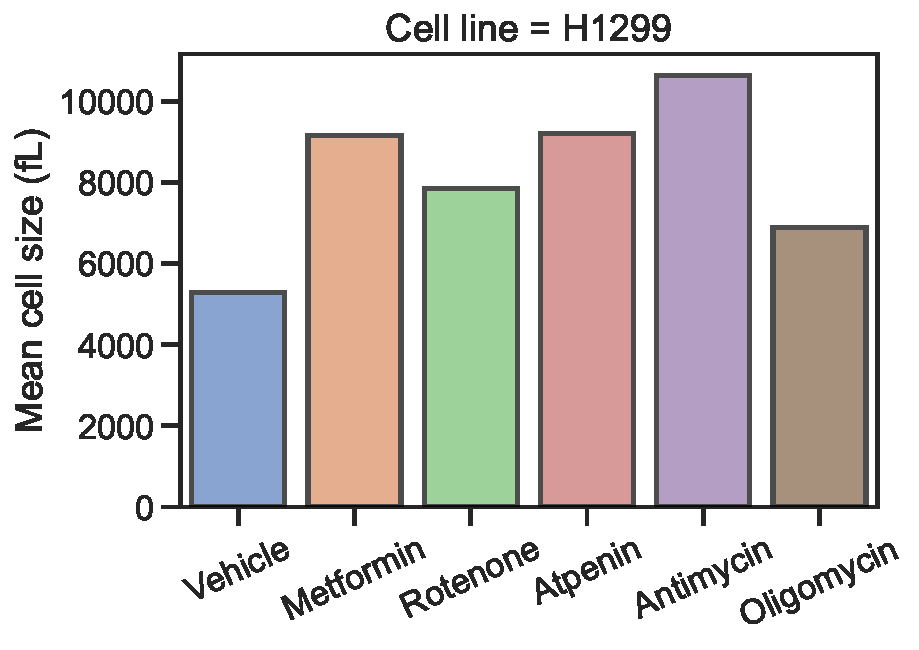
\includegraphics[width=\textwidth]{figures/chap6/ETCinhib_cell_size_H1299.pdf}
     \end{subfigure}
     \begin{subfigure}[b]{0.4\textwidth}
         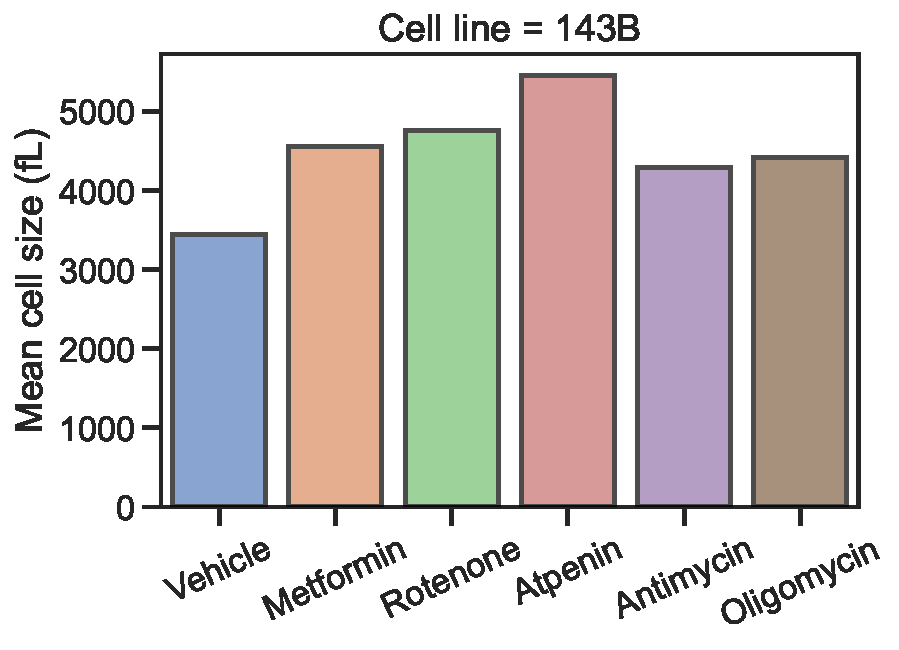
\includegraphics[width=\textwidth]{figures/chap6/ETCinhib_cell_size_143B.pdf}
     \end{subfigure}
        \caption[Mitochondrial inhibitors increase cell size.]{
        A panel of mitochondrial inhibitors all lead to cell size increase in H1299 and 143B cells.
        For H1299 drug treatments: vehicle (DMSO), metformin (6 mM), rotenone (50 nM), atpenin (5 µM, 1 mM pyruvate), antimycin (5 µM) and oligomycin (1 nM).
        For 143B drug treatments: vehicle (DMSO), metformin (2 mM), rotenone (50 nM), atpenin (5 µM, 1 mM pyruvate), antimycin (100 nM) and oligomycin (5 nM).
        Cell size measured using a Coulter counter 3 days after drug treatment.
        }
        \label{fig:ch6:H1299_143B_ETCinhibi_cell_size}
\end{figure}

\begin{figure}
    \centering
    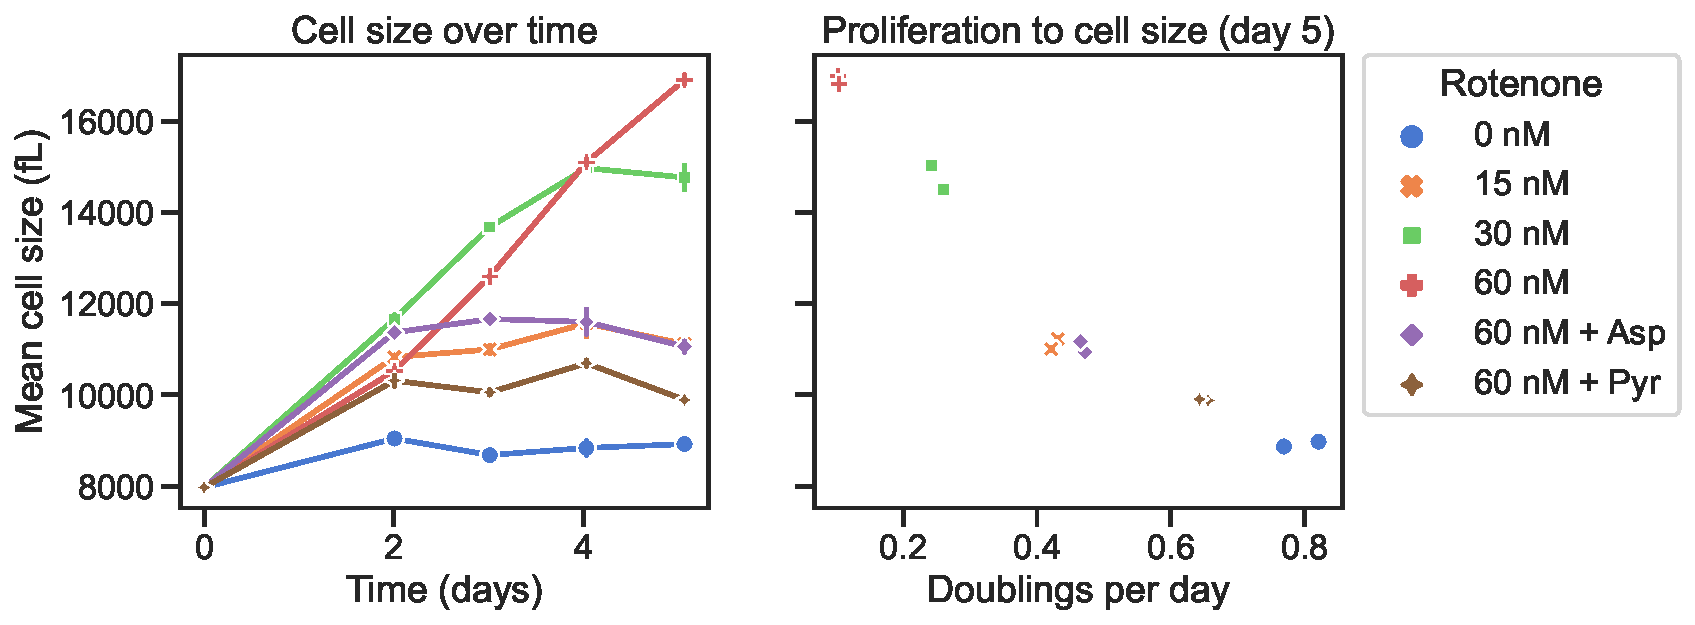
\includegraphics[width=0.8\textwidth]{figures/chap6/cell-size-time_prlfr.pdf}
    \caption[Rotenone induced cell size increase over time.]{
    Rotenone induces an increase in H1299 cell size over time and after 5 days a linear correlation between cell size and proliferation rate is observed.
    Data from replicate 1 proliferation experiment shown in chapter \ref{chap2}, figure \ref{fig:ch2:NAD_Asp_time}.
    }
    \label{fig:ch6:cell_size_time_prlfr}
\end{figure}

\begin{figure}
     \centering
     \begin{subfigure}[b]{0.49\textwidth}
         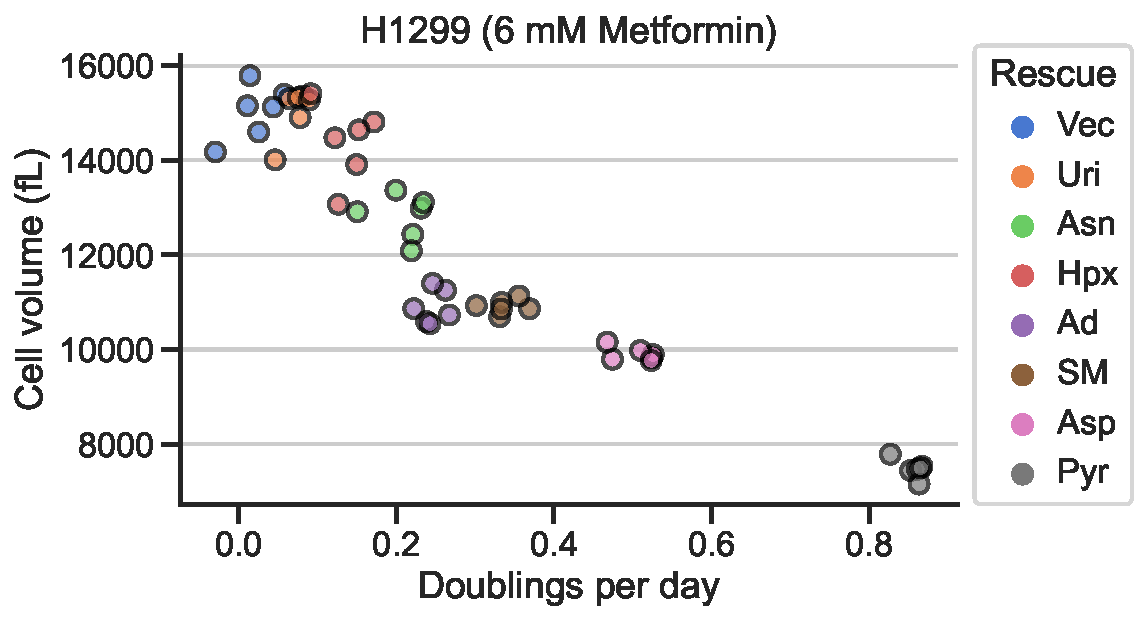
\includegraphics[width=\textwidth]{figures/chap6/H1299_Met_cellvol.pdf}
         \caption{}
         \label{fig:ch6:H1299_Met_cellvol}
     \end{subfigure}
     \hfill
     \begin{subfigure}[b]{0.49\textwidth}
         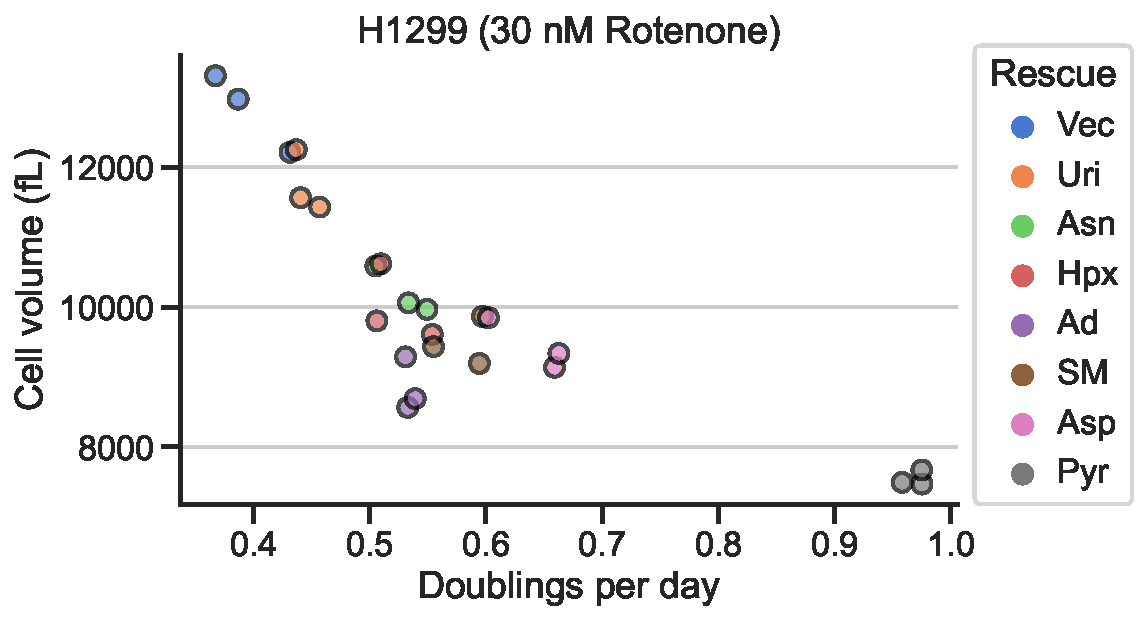
\includegraphics[width=\textwidth]{figures/chap6/H1299_Rot_cellvol.pdf}
         \caption{}
         \label{fig:ch6:H1299_Rot_cellvol}
     \end{subfigure}
        \caption[Proliferation rate correlation with cell volume.]{
        Proliferation rate correlates with cell volume across a panel of metabolites partially rescuing aspartate limitation induced with metformin or rotenone.
        Cell volumes in (a) and (b) from endpoint counts from figures \ref{fig:ch2:H1299_Met_rescue} and \ref{fig:ch2:H1299_Rot_rescue}, respectively.
        }
        \label{fig:ch6:H1299_ETCrescue_vol}
\end{figure}

\begin{figure}
    \centering
    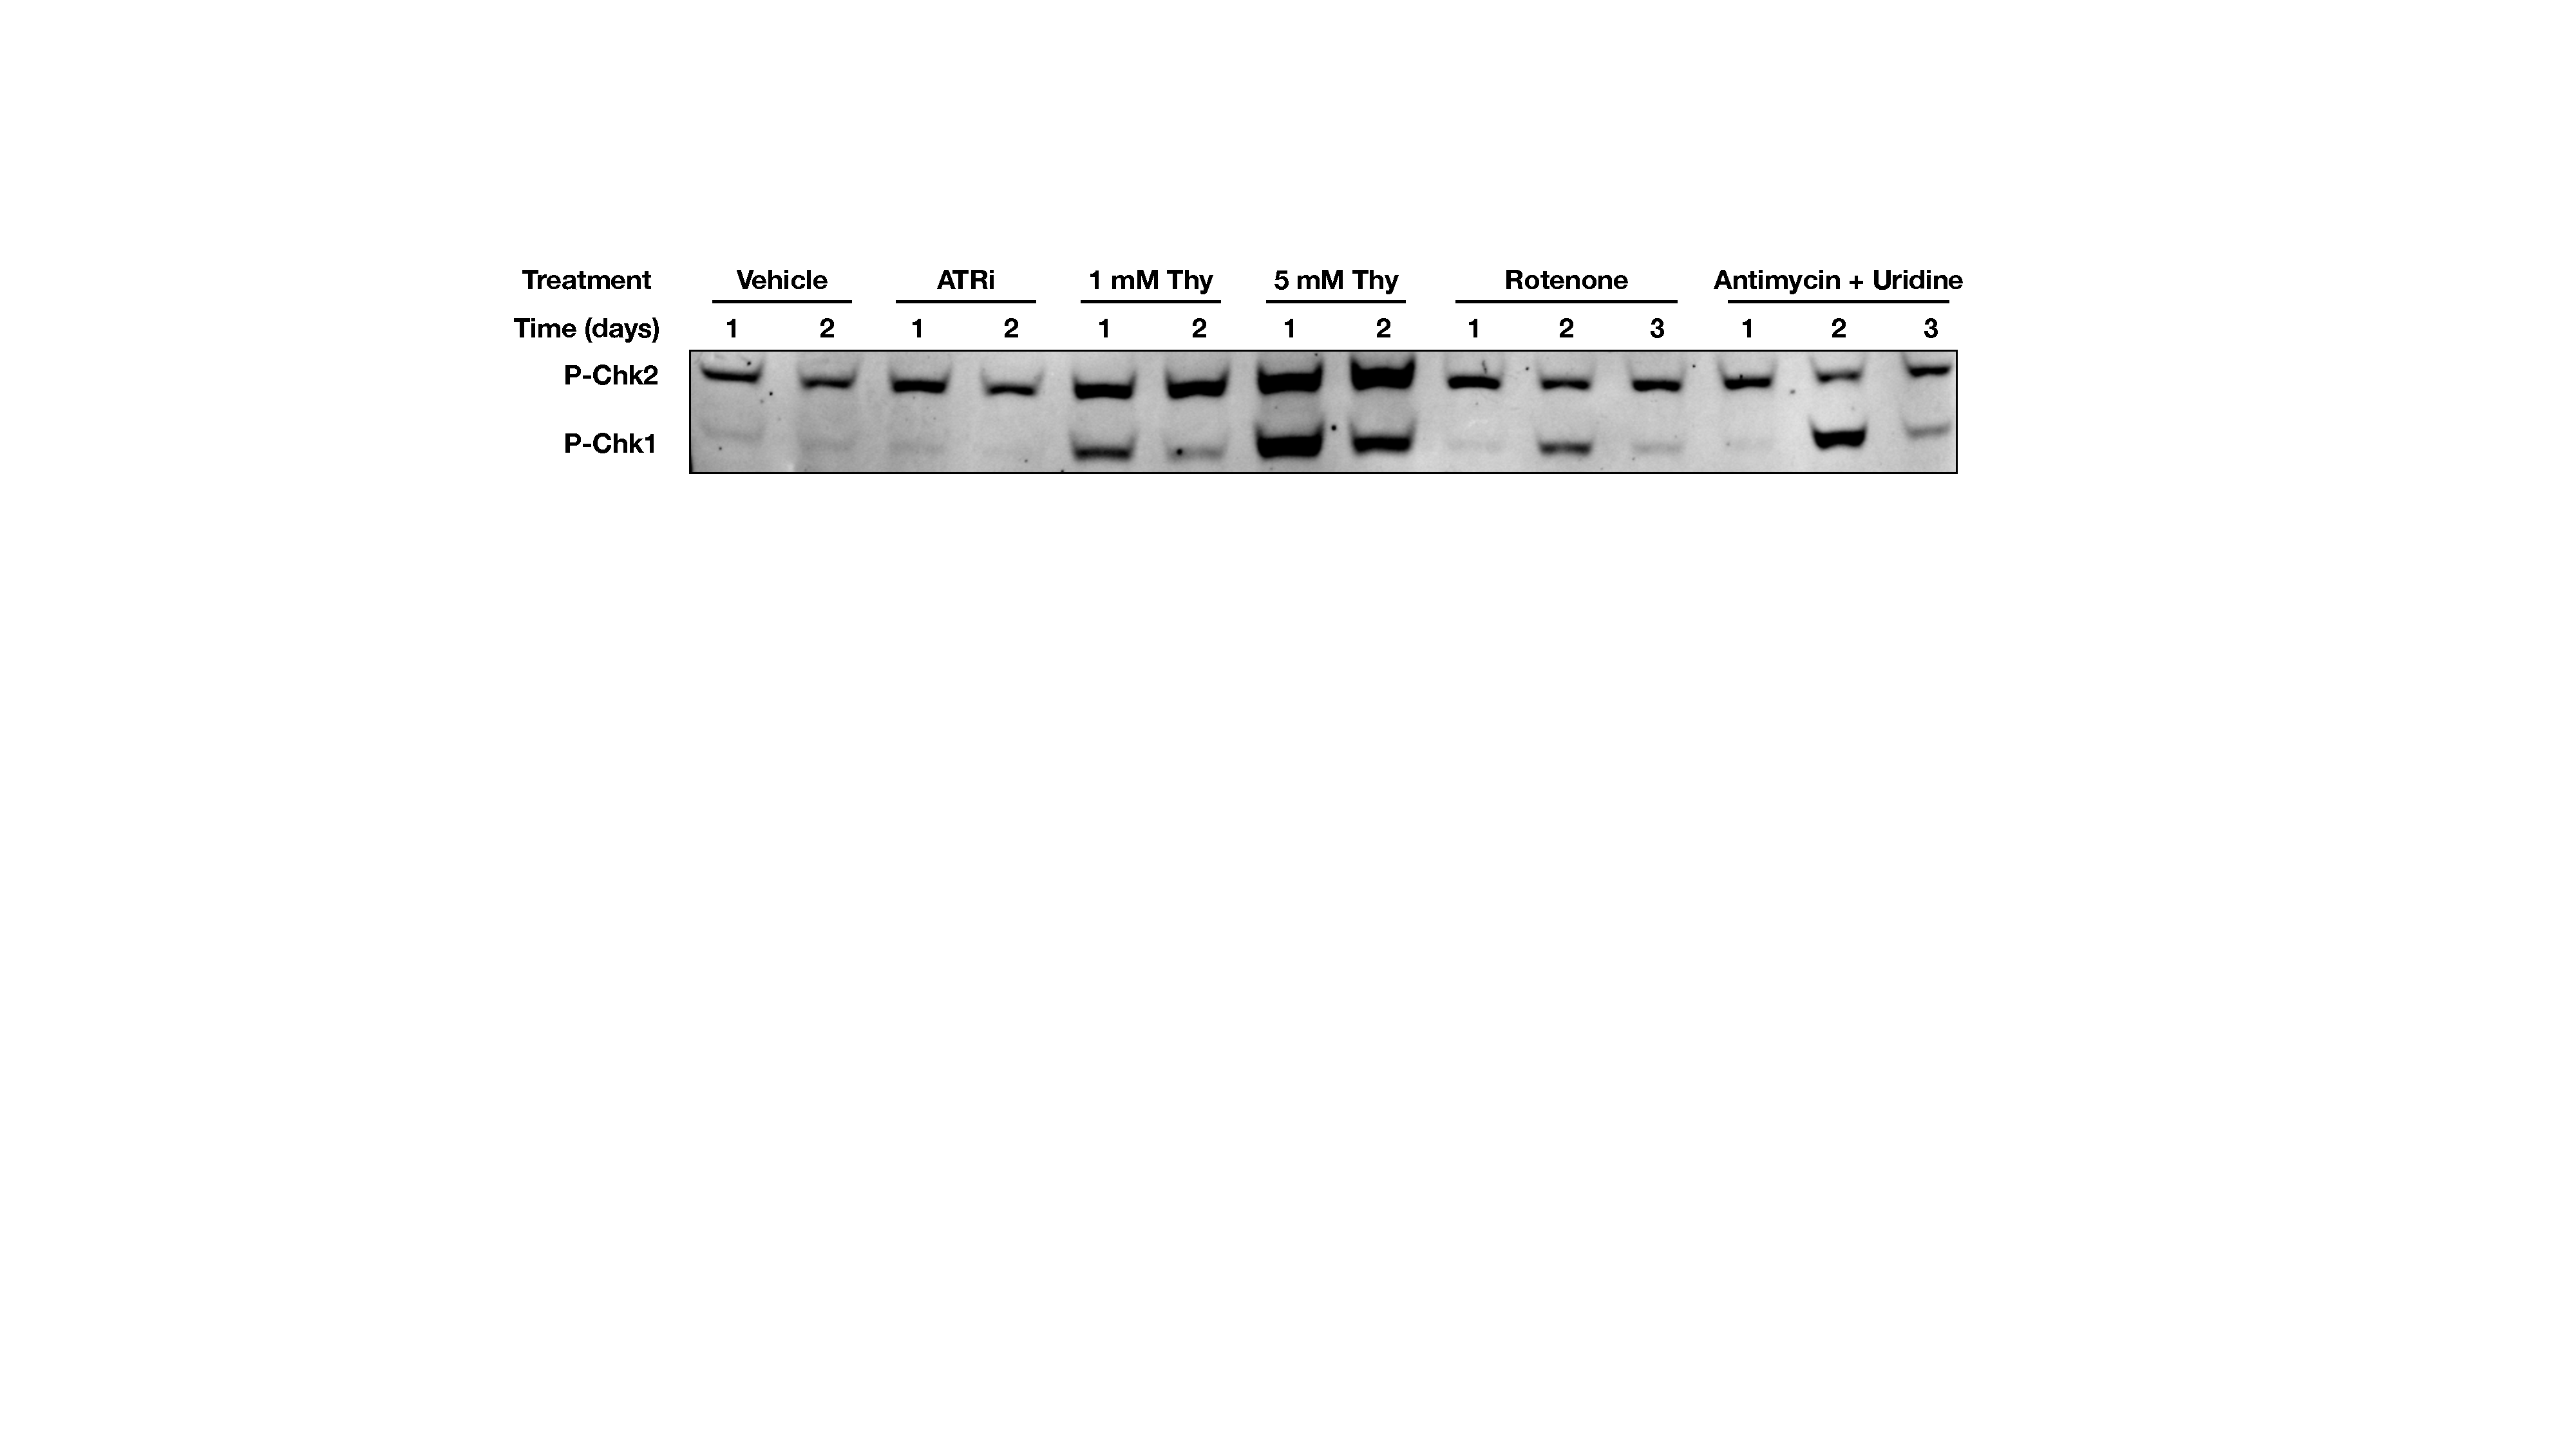
\includegraphics[width=0.7\textwidth]{figures/chap6/P_Chk_wstrn.pdf}
    \caption[Chk1/2 phosphorylation after rotenone/antimycin treatment.]{
    Chk1/2 phosphorylation in H1299 cells over time.
    Treatments: vehicle (untreated), ATRi (50 nM, AZ20), thy (1 and 5 mM thymidine), rotenone (200 nM), antimycin+uridine (5 µM + 200 µM).
    }
    \label{fig:ch6:P_Chk_wstrn}
\end{figure}




\section{Aspartate sensor}
Mass spectrometry is the workhorse for detection and quantification of metabolites because of its unrivaled sensitivity and specificity while maintaining versatility.
But alas, the versatility of measuring thousands of metabolites, is traded for the destructivity of sample ionization.
Protein based sensors offer the inverse trade with sample preservation but low versatility and thus these approaches have the potential of being complementary.

In the study of aspartate limitation, such a biosensor can be a very useful tool.
For example, in parts of chapter \ref{chap2} a hypothesis is put forth about the expected intracellular aspartate level necessary to sustain proliferation with and without salvage complementation of the non-protein fates of aspartate.
To generate these aspartate to proliferation curves, a large number of samples had to be collected and processed for mass spectrometry only to measure aspartate.
Using the aspartate sensor, similar measurements can now be performed with much less work.

Further development and characterization could make this sensor more useful e.g. a better approach to normalization and development of expression systems tested on more cell lines.
While nuclear RFP normalization appears to work quite well in practice, it remains unsatisfactory to normalize to a protein which expression is decoupled from that of the sensor's.
Another unsolved issue is robust sensor expression which was good for some cell lines but poor in others.
In the future, it should be exciting to use the sensor for measurement of compartmentalized aspartate pools; specifically, the mitochondria are relevant due to their role in aspartate synthesis.
A particularly interesting opportunity offered by a biosensor is the ability to combine intracellular aspartate measurements with genetic screening tools.
CRISPR-based screens of gene knockouts and expression induction and suppression have become widely available and often coupled to flow cytometry assisted cell sorting to select for phenotypes other than proliferation.
A similar approach might not be directly applicable for the aspartate sensor because of difficulties preserving intracellular metabolite levels while cell sorting and therefore such an effort may have to use laser tagging to mark the cells before sorting \cite{Binan2016-hn, Hasle2020-vb}.




\section{Further development and applications of tRNA-Seq}
The method presented in chapter \ref{chap5} improves on two main aspects of tRNA-Seq: 1) enabling the measurement of aminoacylation quantitatively and 2) showing that non-heuristic alignment can be applied in practice.
In the limit of perfect alignment performance, heuristic alignment algorithms like Bowtie, BWA, STAR, GSNAP, SHRIMP etc. become equal to the deterministic Smith-Waterman alignment.
The sole reason for using heuristics is to improve efficiency i.e. reduce runtime to a manageable level, which is very important when aligning billions of reads containing hundreds of billions of nucleotides against a 3.2 billion nucleotide genome.
Compare this to tRNA-Seq which produces of few dozen million reads containing a few billion nucleotides that must be aligned against a 40,000 nucleotide tRNA reference set and you get an alignment problem reduced by approximately one million fold.
This, along with continued improvement of CPU speed, makes it possible to use all-against-all Smith-Waterman alignment for tRNA-Seq data.
So, it is possible, it has a clear theoretic justification and it can even be used in practical settings, but is it necessary?
The question is not answered in chapter \ref{chap5} and currently there is no good benchmark.
A good approach for such benchmark would be a simulation study to establish a ground truth and test the influence of the various parameters e.g. RT-PCR readthrough, tRNA modifications, reference set size etc.
A tRNA-Seq read simulator was actually made and is available on Github (\href{https://github.com/krdav/tRNA-charge-seq/blob/8a096d023d19dd8e6419460d72c1ea4051ffd64d/utils/code-of-limited-use/tRNA-Seq_simulator.ipynb}{link}).

Since our method was submitted, another tRNA-Seq method was published by Sun et al. \cite{Sun2023-sx}.
Herein they use nanopore sequencing to generate reads but otherwise their data is like that generated using Illumina sequencing.
They reach a similar conclusion regarding alignment and substantiate it by pointing to examples of misalignment when using BWA.
These misalignments were caused by the high degree of RT-PCR generated misincorporations and could be resolved using Smith-Waterman alignment.
Furthermore, they employ a statistical model to infer tRNA modifications from RT-events.
This can be advantageous because it offers a principled way of comparing differences in tRNA modification status e.g. as a response to nutritional change, drug treatments etc.
Another way of modelling these RT-events would be as a Markov chain in which the tRNA modification probabilities would be described by a hidden Markov model \cite{durbin1998biological}.

On the chemistry side of things there are many possible improvements to be made.
Past efforts have been made to improve RT-PCR readthrough, but these are far from exhaustive.
Therefore, there is an opportunity to systematically test different RT polymerases, buffers, temperatures and other incubation conditions.
It may even be possible to couple these tests to a selection method and develop a screen.
If successful, a better readthrough would have a large impact on the method by improving read mapping and expanding the coverage of inferred tRNA modifications.
Improved and expanded detection of tRNA modifications could also be achieved by using chemical treatments to ``activate'' a modified residue, thereby enhancing its propensity to generate an RT-event as observed for periodate treated 2-thiouridine residues.
With efforts to improve detection of tRNA modifications, it will be important to control for batch variations impacting the likelihood of an RT-events, for example small difference in reagents like the dNTP concentration, RT-polymerase, buffers etc.
An internal control could be devised and used similarly as the spike-in controls already employed.
A convenient source for such control is \textit{E.coli} isolated tRNA, since it has relatively few tRNA transcripts that are all easily distinguishable from human tRNA transcripts.
As a control, it would be isolated once and added in small amounts to all samples.
The RT-event pattern of the \textit{E.coli} tRNA transcripts would be expected to remain constant across all samples and thus samples with large deviations could be flagged and discarded.

Regarding applications, it would be highly useful to test the method with tissue samples.
There is no reason why the method should not be able to work with tissue; however, testing is warranted due to potential issues with glycogen contamination resulting in quenching of the periodate oxidation.
With tissue samples, it would be interesting to first survey tRNA charge, expression and modifications across different organs or cell types, particularly those engaged in high protein expression such as pancreatic, endocrine and lymphoid tissues.
Thereafter, the method could be applied to tissues from diseases related to defects in amino acid metabolism and/or translation.

Accurate quantitative tRNA charge measurements also enable several assay developments.
For example, when used in conjunction with expression of a library of tRNA sequences, it could be applied to better identify the tRNA sequence requirements of aminoacyl tRNA synthetases.
Some of the tRNA elements that specify aminoacylation specificity have already been identified, but with a high-throughput method the resolution of these could greatly increase.
The aminoacylation specificity can be described as a tRNA sequence's ability to be aminoacylated or not; however, a better description would be to quantify the changes in the enzyme kinetic parameters.
This may be possible by taking measurements over time to make a set of progress curves from which kinetic data can be extracted using numerical integration \cite{Johnson2009-cx, Johnson2013-df}.
Finally, tRNA-Seq can accelerate the development of non-canonical tRNA:aminoacyl tRNA synthetases pairs in several ways.
For example, by identification of tRNAs that are compatible with host tRNA processing, while only being aminoacylated upon expression of the cognate aminoacyl tRNA synthetases and not by native host enzymes. 

